\documentclass[sigconf]{acmart}
\settopmatter{printacmref=false, printccs=false, printfolios=true}
\renewcommand\footnotetextcopyrightpermission[1]{}


\usepackage{booktabs} % For formal tables


%%%%%
\usepackage{listings}
\usepackage{xcolor}

\definecolor{codegreen}{rgb}{0,0.6,0}
\definecolor{codegray}{rgb}{0.5,0.5,0.5}
\definecolor{codepurple}{rgb}{0.58,0,0.82}
\definecolor{backcolour}{rgb}{0.95,0.95,0.92}

\lstdefinestyle{mystyle}{
    backgroundcolor=\color{backcolour},   
    commentstyle=\color{codegreen},
    keywordstyle=\color{magenta},
    numberstyle=\tiny\color{codegray},
    stringstyle=\color{codepurple},
    basicstyle=\ttfamily\footnotesize,
    breakatwhitespace=false,         
    breaklines=true,                 
    captionpos=b,                    
    keepspaces=true,                 
    numbers=left,                    
    numbersep=5pt,                  
    showspaces=false,                
    showstringspaces=false,
    showtabs=false,                  
    tabsize=2
}

\lstset{style=mystyle}

\begin{document}
\title{Concurrency and Parallelism Project}


\author{Guilherme Fernandes}
\email{60045}

\author{Vladyslav Mikytiv}
\email{60735}


\begin{abstract}
This report provides the explanation and the implementation of parallelisation of the algorithm of equalization of images. Both an OpenMP and CUDA implementations.

\end{abstract}

% We no longer use \terms command
%\terms{Theory}

\keywords{OpenMP Parallelism C++ CUDA}


\maketitle

\section{Critical Code Analysis and Parallelization}
\subsection{The first steps}

At first we ran the code without doing any modifications and used the profiler in order to identify the hot spots doing a average value in each image of the time lost in functions from the profiler. The algorithm runs for 100 iterations.

\begin{table}[h!]
\centering
\begin{tabular}{|c|c|}
\hline
\textbf{Function} & \textbf{Computation Time Lost (\%)} \\
\hline
correctColor\&rescale & 57.98\% \\
\hline
grayScale & 23.17\% \\
\hline
normalize & 18.24\% \\
\hline
\end{tabular}
\vspace{0.2cm} % Adjust the space here
\caption{Average Computation Time Lost in Functions}
\label{table:computation_time_lost}
\end{table}
As seen in Listing \ref{table:computation_time_lost} the zones of the code that took a long time to perform the computation and in overall slow down the algorithm are:
the \textbf{\texttt{normalization}} of the image, the \textbf{\texttt{correction of color}}, the \textbf{\texttt{convertion to the greyscale}} and some other
not so computational heavy functions.


 To reduce the impact on processing time caused by these functions within the algorithm, we integrated OpenMP directives into these specific parts of the code to accelerate computation.
 
 It's important to highlight the \textbf{thread management}. Since we are working with images we will have to do some simples calculus to determine the amount of work that
 each thread will be given. For that we must perform two calculations (one for RGB and one for the grey scale). For the RGB  we will calculate $\texttt{WIDTH * HEIGHT * 3}$ and to obtain the \texttt{CHUNK\_SIZE\_RGB} we just divide $\texttt{WIDTH * HEIGHT * 3}$  by \texttt{N\_THREADS}. For the grey scale it's similar but we don't multiply by 3 getting the \texttt{CHUNK\_SIZE}. Now we will have the work that will be balanced between threads.
 
\subsection{\textbf{Function parallelization}}

The \textbf{normalization} function will be improved with the following code: \texttt{\textbf{pragma omp parallel for}} with the option \texttt{\textbf{schedule(static, chunk\_size\_channels)}} and \texttt{\textbf{num\_threads(n\_threads)}}. This code optimization can be seen in Listing \ref{lst:normalization_function}.

\begin{lstlisting}[language=C, caption=Normalization Function, label={lst:normalization_function}]
void normalize(//omitting for space) {
    #pragma omp parallel for schedule(static, chunk_size_channels) num_threads(n_threads)
    for (int i = 0; i < size_channels; i++)
        uchar_image[i] = (unsigned char) (255 * input_image_data[i]);
}
\end{lstlisting}
The \textbf{grey scale conversion} will be improved in two ways. We will mix the \texttt{fill\_histogram}
function with this one in order to do everything in the same function. Besides that we also apply the following OpenMP directives: \texttt{\textbf{pragma omp parallel for}}
with the option \texttt{\textbf{reduction(+:histogram)}} and \texttt{\textbf{num\_threads(n\_threads)}}. This code optimization can be seen in Listing \ref{lst:gray_function}.
\begin{lstlisting}[language=C, caption=Grey Conversion Function, label={lst:gray_function}]
	void convertoToGrayScale(//omitting for space) {
       	// filling the histogram with zeroes
        #pragma omp parallel for reduction(+:histogram) num_threads(n_threads)
        for (int i = 0; i < size; i++){
                auto r = uchar_image[3 * i];
                auto g = uchar_image[3 * i + 1];
                auto b = uchar_image[3 * i + 2];
                gray_image[i] = 
                static_cast<unsigned char>
                (0.21 * r + 0.71 * g + 0.07 * b);
                histogram[gray_image[i]]++;
            }
    }
\end{lstlisting}
We can't parallelize the \textbf{CDF calculcation} because it has true dependencies between iterations and also it's not worth due to the number of iterations (256).
Another function that we managed to simplify was the \texttt{cdf\_min\_loop}. Since we minimum will always be on the first position we just return it and that's how we compute
the minimum of the CDF.

The \texttt{\textbf{correct\_color\_loop}} can be mixed with the \texttt{\textbf{rescale}} following the same strategy as we did with \texttt{grey scale} and \texttt{fill historgram} functions. The code optimization is the same as Listing \ref{lst:normalization_function} and can be seen in Listing \ref{lst:correct_function}.
\begin{lstlisting}[language=C, caption=Color Correction Function, label={lst:correct_function}]
	void correct_color_loop_and_rescale(//omitting for space) {
        #pragma omp parallel for schedule(static, chunk_size_channels) num_threads(n_threads)
        for (int i = 0; i < size_channels; i++)
        {
            uchar_image[i] = correct_color(cdf[uchar_image[i]], cdf_min);
            output_image_data[i] = static_cast<float>(uchar_image[i]) / 255.0f;
        }
    }
\end{lstlisting}
\subsection{Decions}
It's important to justify our reasoning. We used \texttt{\textbf{static}} in every single call of the OpenMP directives because the extra overhead of orchistrating the threads with a certain amount of work did not compensate. As we can see in the Table \ref{table:staticanddynamic} \texttt{\textbf{static}} always shows better results and it's coherent to the theoretical analysis. For this simulation we used 16 threads and 100 iterations.

\begin{table}[h!]
\centering
\begin{tabular}{|c|c|c|}
\hline
\textbf{Dynamic Time (ms)} & \textbf{Static Time (ms)} & \textbf{Image Name} \\
\hline
117 & 99& borabora.ppm \\
\hline
98 & 81 & input01.ppm \\
\hline
5620 & 4369 & sample.ppm \\
\hline
\end{tabular}
\vspace{0.2cm} % Adjust the space here
\caption{Dynamic vs Static Mean Execution Times}
\label{table:staticanddynamic}
\end{table}

\section{Metric Analysis - OpenMP}
Now, let's assess the impact of these changes on the runtime of our program. For that we will use \textbf{speed up} and \textbf{efficienty} and we will execute every executing multiple times in order to get the mean value of the execution times.

The code was in a cluster executed with the following specifications: \textbf{2x Intel Xeon E5-2609 v4}, with \textbf{16 cores} and \textbf{NVIDIA Quadro M2000} GPU.

\begin{figure}[h]
  \centering
  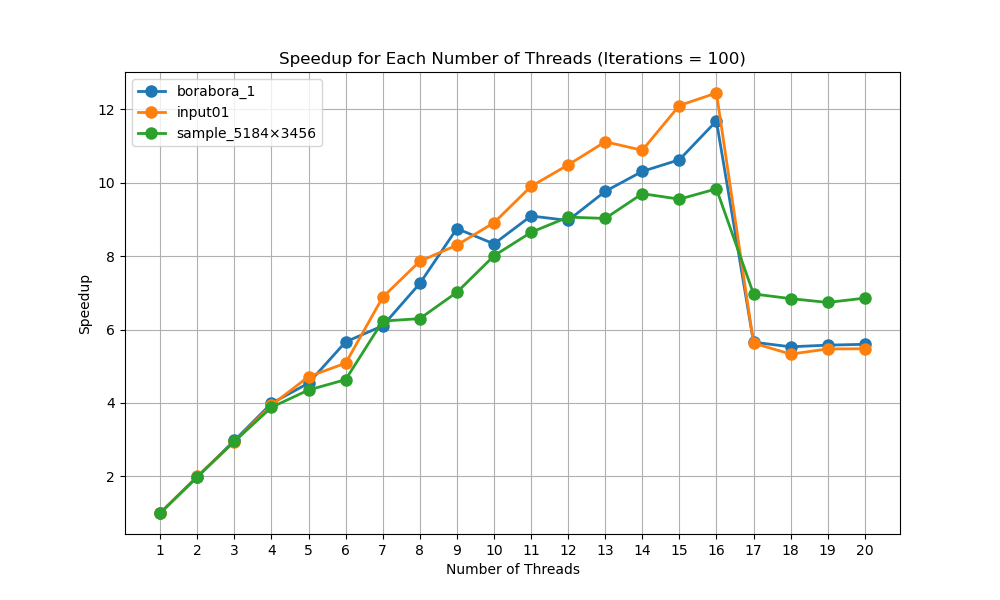
\includegraphics[width=\linewidth]{images/openMP.png}
  \caption{Speedup across different number of threads usage of different images}
 \label{fig1}
\end{figure}

Figure \ref{fig1} describes the speed up for the different images in our test set. We can clearly see a rise on the speed up until a certain point. After that point the value of the speed up begins to decrease. The optimal \texttt{NR\_THREADS} to perform the computation is 16.

In order to calculate the efficiency we will use the best result that we had: the one with 16 threads. For that we define $S_{16}$ which is the speed up with 16 threads and it will be equal to $$S_{16} \approx 11$$

And the efficiency of the parallelel implementation in Section 1 get's us an efficiency value of: $$E_{16} = \frac{S_{16}}{16} \approx 69\%$$

\section{CUDA}
We've attained speed enhancements leveraging the OpenMP library for parallelizing our code. However, there exists an avenue to further escalate our computational efficiency. By harnessing the GPU architecture through CUDA, we can unlock additional acceleration potential.

To leverage the GPU effectively, we need to define kernels for specific regions of our code that we wish to offload to the GPU for computation. This necessitates defining grids use in CUDA kernels.

Utilizing the GPU for optimization involves creating kernels to transfer data to the GPU, perform computations, and retrieve the results back to the CPU. Given the high cost associated with these operations, minimizing the number of kernels is imperative. After several iterations, we've determined that the minimum number of kernels required is three. Due to dependencies, namely the need for histogram calculation in operations like correcting colors and resizing, we cannot combine the first kernel with the third one.

The initial kernel handles both the normalization and grayscale operations. Since these operations are independent of each other, we can consolidate them into a single kernel instead of creating two separate ones. The Listing \ref{lst:gray_norm_function} shows this kernel implementation.

\begin{lstlisting}[language=C, caption=Grey Conversion and Normalization, label={lst:gray_norm_function}]
__global__ void normalize_kernel(//omitting for space) {
        int ii = blockIdx.y * blockDim.y + threadIdx.y;
        int jj = blockIdx.x * blockDim.x + threadIdx.x;
        int idx = (ii * width + jj)*3;

        if (ii < height && jj < width) {
            for(int i = 0; i < 3; i++) {
                // Normalize logic
            }
            auto r = uchar_image[idx];
            auto g = uchar_image[idx + 1];
            auto b = uchar_image[idx + 2];
            idx =ii * width + jj;
            gray_image[idx] = // Calculation
        }
    }
\end{lstlisting}

Before proceeding to the second kernel, it's essential to calculate the histogram. While we could create a custom kernel for this task, a more efficient approach involves leveraging the \texttt{\textbf{CUB}} library. By utilizing its operations, we can significantly enhance the performance of our code.

By using \texttt{\textbf{cub::DeviceHistogram::HistogramEven}} we are able to calculate the histogram in the GPU without making the kernel ourselves.

After having the histogram we can calculate the probabilities in order to use them in another call to the \texttt{\textbf{CUB}} library. For that we create a second kernel, which will seem more clear why ahead. This one will differ from the first one in the \texttt{\textbf{numBlocks}} and \texttt{\textbf{blockSize}}. The \texttt{\textbf{numBlocks}} will be $256$ and the \texttt{\textbf{blockSize}} will be \texttt{(HISTOGRAM\_LEN+ blockSize-1) / blockSize}.

Once we have computed this probability array, we can further utilize it in another function provided by the \texttt{\textbf{CUB}}  library.

The \texttt{\textbf{cub::DeviceScan::InclusiveSum}} function facilitates the calculation of the final cumulative distribution function (CDF) values. This not only streamlines the programming process but also optimizes computation time, offering significant efficiency gains. We used the \texttt{\textbf{InclusiveSum}} because it was not possible to use \texttt{\textbf{cub::DeviceScan::InclusiveScan}} due to restrictions in the library (there was no way to pass the probabilities to this call). That's why we must calculate the probabilities beforehand and use the \texttt{\textbf{InclusiveSum}}.

Ultimately, we employ our final kernel, which could theoretically be executed within the first kernel. However, due to dependencies necessitating separate execution, we're compelled to create this third kernel to handle the last part of the algorithm. The code can be seen in Listing \ref{lst:last_func}.

\begin{lstlisting}[language=C, caption=Correct and Rescale, label={lst:last_func}]
 __global__ void correct_kernel(//omitting for space) {
        int ii = blockIdx.y * blockDim.y + threadIdx.y;
        int jj = blockIdx.x * blockDim.x + threadIdx.x;
        int idx = (ii * width + jj)*3;

        if (ii < height && jj < width) {
            for (int i = 0; i < 3; i++) {
                auto cdf_val = d_cdf[uchar_image[idx+i]];
                float cdf_min = d_cdf[0];
                
                uchar_image[idx+i] = // Logic

                output_image_data[idx+i] = // Logic
            }
        }
    }
\end{lstlisting}
These kernels constitute the entirety of the GPU-accelerated operations. Due to space constraints, significant portions of the code have been omitted. For the complete implementation, please refer to the accessible code at \url{https://github.com/Gui28F/CP-Project}. 

\section{Metric Analysis - CUDA}
Utilizing the capabilities of the GPU necessitates defining the grid dimensions. To determine the optimal \texttt{TILE\_WIDTH} value, we conducted an experiment, the results of which are depicted in Figure \ref{fig2}. It was discerned that the most favorable value was 16. Notably, we are constrained from exceeding 32 due to the limitation imposed by the maximum thread utilization, capped at $32 * 32 = 1024$.

\begin{figure}[h]
  \centering
  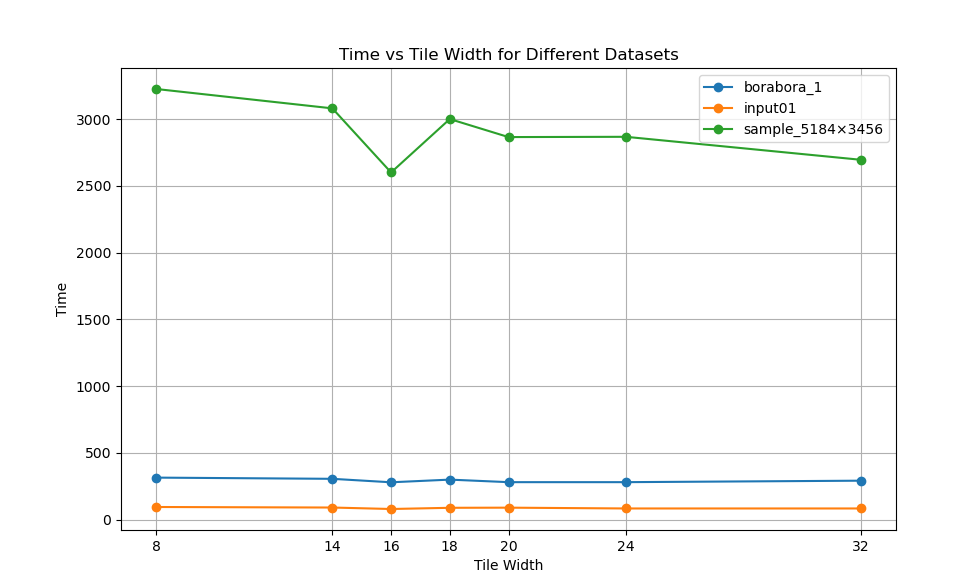
\includegraphics[width=\linewidth]{images/tilesss.png}
  \caption{Tiles Width and Execution Time}
 \label{fig2}
\end{figure}
To effectively evaluate the performance of the GPU-accelerated version, it's important to compare it against the most optimized configuration achieved with OpenMP (specifically, the one utilizing 16 threads). Figure \ref{fig3} illustrates the differences in speedup compared to the optimal OpenMP configuration.

\begin{figure}[h]
  \centering
  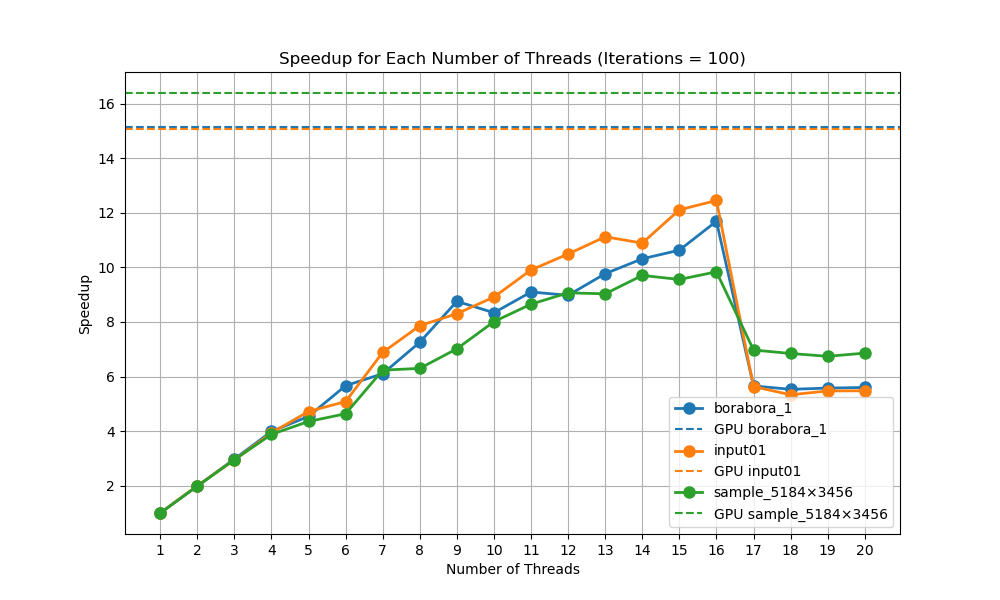
\includegraphics[width=\linewidth]{images/openMPCUDA.png}
  \caption{OpenMP vs CUDA}
 \label{fig3}
\end{figure}




\section{Final Results}
After implementing optimizations using \textbf{OpenMP} and \textbf{CUDA}, we now have a clearer understanding of the overall performance. The table presents execution times for the purely sequential implementation, the \textbf{OpenMP} implementation, and the \textbf{CUDA} implementation. These results, obtained from 100 iterations of the algorithm, represent the mean calculated values derived from running the algorithm five times.The names were shortened in the table \footnote{\textbf{Description:} SQT -- Sequential Time, OMPT -- OpenMP Time, CUDAT -- CUDA Time}.

Each generation of results was derived from the average of five separate runs the algorithm with 100 iterations. By calculating the mean of these five separate executions, we aimed to obtain more reliable and trustworthy results. This approach ensured that our findings were not skewed by anomalies in any single run, providing a more accurate representation of the algorithm's performance.

\begin{table}[h!]
\centering
\begin{tabular}{|c|c|c|c|}
\hline
\textbf{SQT (ms)} & \textbf{OMPT (ms)} & \textbf{CUDAT (ms)} & \textbf{Image} \\
\hline
1140 & 98 & 76 & borabora.ppm \\
\hline
956 & 76 & 63 & input01.ppm \\
\hline
10943 & 4371 & 2635 & sample.ppm \\
\hline
\end{tabular}
\vspace{0.2cm} % Adjust the space here
\caption{Final Execution Times}
\label{table:staticanddynamic}
\end{table}

\section{Tests}
During the development we guided ourselves with the GoogleTest for both the OpenMP and CUDA implementations. With these tests we are sure that the pixels of the resulting images are correct and not just visually correct by looking at the images. The test files are also available on the GitHub repository.

\section{Conclusions}
Whether through the integration of OpenMP directives or harnessing the power of GPU acceleration, we consistently observe improved results compared to the raw sequential implementation. Notably, in the case of the borabora.ppm image, an anomaly surfaces where the OpenMP implementation slightly outperforms the CUDA counterpart. We attribute this discrepancy to potential pixel saturation issues. Nonetheless, it's important to note that, in general, the CUDA implementation remains the preferred choice, with ongoing comparisons against OpenMP to ensure optimal performance.

\section{Code}
All the code mentioned above can be consulted in \url{https://github.com/Gui28F/CP-Project}.
\section{Individual Contribution and Comments}
The project was a joint effort, with both team members sharing the workload equally. We utilized pair programming sessions on Discord calls and in the lab to accomplish our tasks effectively. We are grateful to Professor Hervé for his invaluable support and constant availability to assist us throughout the project.
\bibliographystyle{acm}
\bibliography{refs}

\end{document}